\part{State of the art} \label{part:state_art}

\chapter{What is the Internet of Things?}

The Internet of Things or IoT, also called Internet of Everything, Web of Things, can be viewed as the interconnection of things, often referred as objects, motes or smart objects. The Global Standards Initiative on Internet of Things (IoT-GSI) defined \textit{Internet of Things} as "\textit{a global infrastructure for the information society, enabling advanced services by interconnecting (physical and virtual) things based on existing and evolving interoperable information and communication technologies}" \cite{ituitu}. They also give an explanation about what they consider a \textit{"thing"} to be. A thing is "\textit{an object of the physical world (physical things) or the information world (virtual things), that is capable of being identified and integrated into communication networks}" \cite{ituitu}.\\

With the IoT, we dispose of networks constituted by devices which have the ability to communicate between them to exchange data. Also, those devices can interact with their environment with the means of sensors or actuators. An illustration of such network would be the \textit{Smart Home}. With Smart Home, automation comes into our house. The idea is to have, for example, your door communicating to the lights to tell them to light on or to light off depending on if you enter or leave the room. You could have your alarm tell the coffee machine to prepare some coffee when ringing in the morning or that your thermostat would regulate the heat of the house. You could also remotely manage your house by activating or deactivating the heat and so on. While discussing the presence of the IoT in homes, one field that could largely benefit from the IoT is the field of \textit{e-health}, thanks to the medical monitoring of elderly, ill, and disabled patients, while they would still be in their house and keep their autonomy in their daily life. Smart objects could either be implanted in or around the patient, and information is retrieved from their situation to have regular checkups on their condition(s). The information is then sent and analyzed by specialized staff, ready to intervene if needed. The advantage here is having the ability to remotely monitor patients' situation.\\

But the IoT is not limited only to home. It is already deployed on organizations. For example, the start-up Epicenter injects microchips into their employees (after agreement)\cite{website:lat_04_17}. The microchip enables an employee to open a door or to operate a printer by just a wave of the hand. It also permits to track them inside the building and allows a colleague to know your whereabouts. \\

The Internet of Things can also be used in many more situations. Power grids can now be better controlled and managed with smart objects, the temperature in buildings and houses can now be monitored and smart objects control radiators and air conditioners to modify ambient temperature, and thus make a more efficient consumption of energy. Shipping containers could also be equipped with devices to better help monitor and modify the climate inside, thus making sure food, clothing, and various materials are better taken care of. Environments hard to analyze like glacier or mountains become easier to monitor as we only need to place sensors nodes that will periodically send us the data retrieved from the environment such as temperature. \\

Those examples show how much we could benefit from IoT. It could improve our efficiency in terms of energy but also in terms of production. But also could make our life easier by automating certain aspects of the life. In the following subsections, we will go deeper into some technical aspects of the Internet of Things. \\

\section{Smart Objects}

Smart objects are the main components of an IoT Network. We will explain what makes them special and the purpose of their use.\\

Smart objects, also called IoT Devices, smart devices or connected devices, are physical objects, that are embedded with an electronic component, that allows them to communicate with other objects. Those objects are composed of a software, are equipped with a microprocessor, a sensor or an actuator that allows them to interact with the physical environment and modify/control it, and network connectivity to allow exchange and collection of data. Thanks to network connectivity, devices can sense and exchange sense data of the physical world with each other. They are also often equipped with a small battery, that provides a power source to the device. The connectivity is assured by wireless in most cases. Fig.\ref{fig:smart_objects} shows examples of smart objects.\\

\begin{figure}
    \centering
    \begin{subfigure}[b]{0.3\textwidth}
        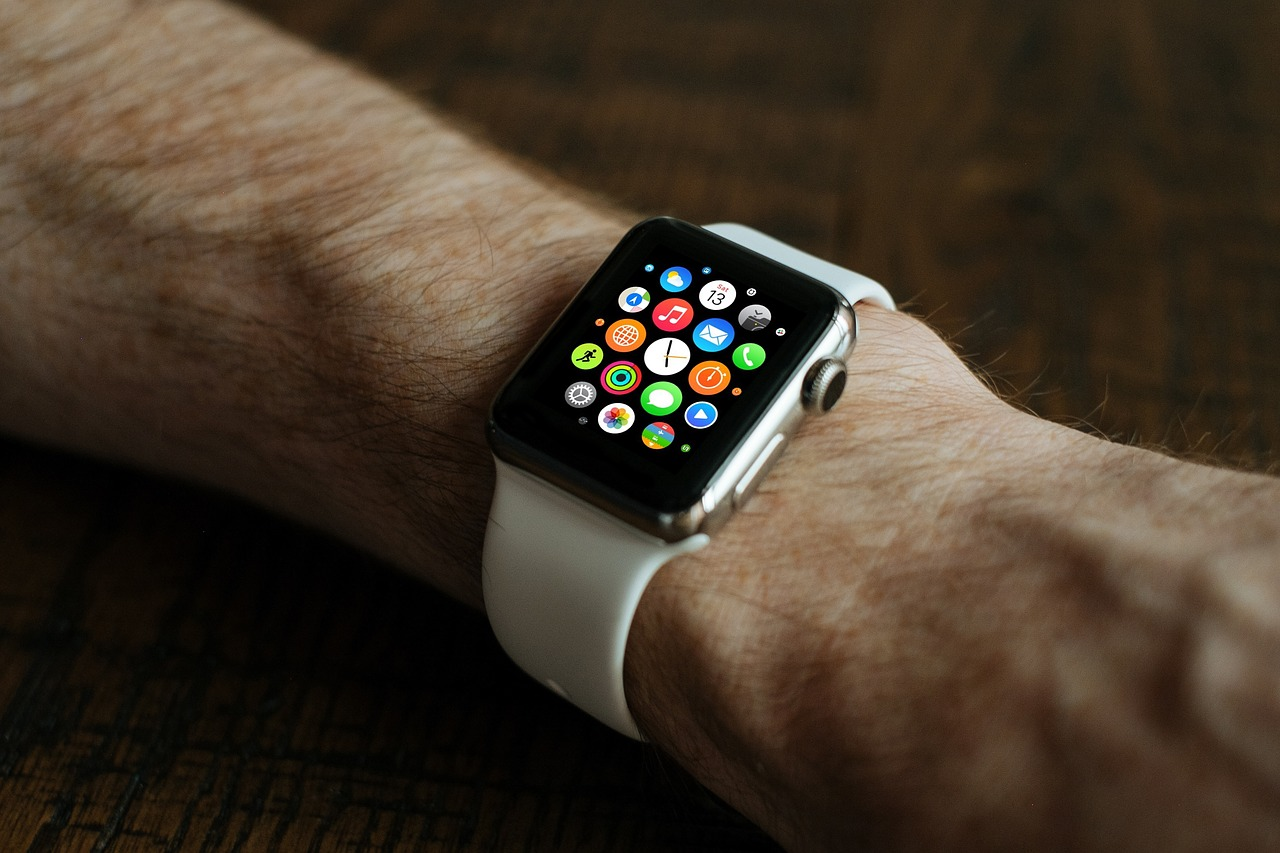
\includegraphics[width=\textwidth]{res/smart_watch}
        \caption{A smart watch}
        \label{fig:smart_watch}
    \end{subfigure}
    ~
    \begin{subfigure}[b]{0.3\textwidth}
        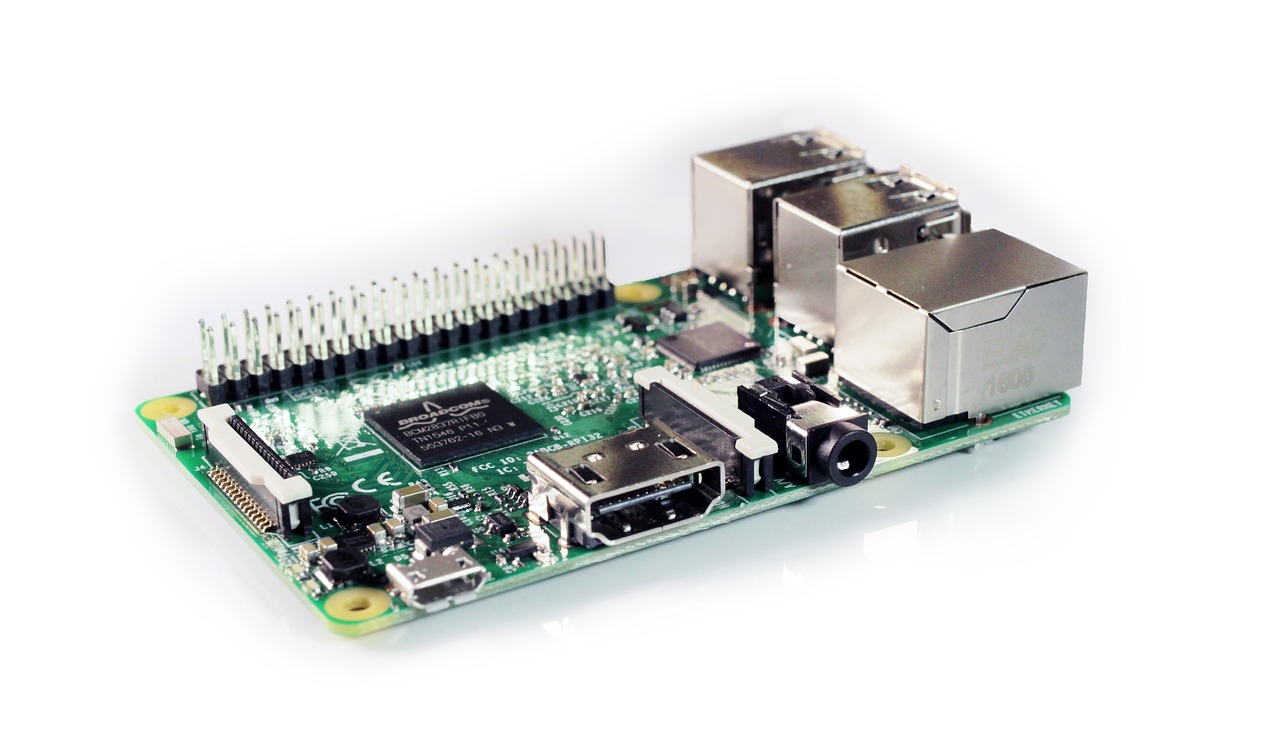
\includegraphics[width=\textwidth]{res/raspberry_pi}
        \caption{A raspberry pi}
        \label{fig:raspberry}
    \end{subfigure}
    \caption{Smart objects (Source: \url{pixabay.com})}\label{fig:smart_objects}
\end{figure}

While it seems pretty straightforward, there does not seem to be a fine line of what exactly "smart objects" refer to. They may refer to the actual small device with processing and interacting capacity, or the bigger entity that is a physical object made "smart" by the addition of a sensor or actuator. In our case we will consider the latter definition of what an IoT device is.
Moreover, in this thesis we will often employ the terms motes, nodes, devices, smart objects or things interchangeably. \\

Those devices are quite limited also in term of resources. They are small embedded devices with low power cpu and a limited memory size. Notably, they are not plugged, meaning they rely mainly on their battery. To maximize the battery lifetime, they often switch between \textit{awake} phases, where the mote is able to communicate and execute process, and \textit{sleep} phases, where the mote does nothing and remains idle. Additionally, their wireless range does not allow them to often communicate directly with all members of the network. This is why most of the IoT networks are organized in a \textit{hop-by-hop} fashion. \\

Tab.\ref{tab:sensors_char} gives some component characteristics about some devices. The raspberry pi 3 presents good specifications. This is typically the type of device that would be used as a sink node or data aggregator or data analyser inside an IoT network. The other devices, the MTM-CM5000-MSP and Zolertia Firefly, are mainly sensor motes. They are used to sense the environment and transmit the values. They are not intended for intensive applications. They do not need high specifications and this is why they present low characteristics compare to the Raspberry. But when designing protocols for the Internet of Things, it is those low power devices that must be taken into account as they are the most restraining. \\

\begin{table}
  \centering
  \begin{tabularx}{\textwidth}{|X|X|X|X|}
    \hline
    Model & MTM-CM5000-MSP & Zolertia Firefly & Raspberry pi 3 \\ \hline
    CPU & 8MHz MSP430 & 32MHz ARM Cortex-M3 & 1.2GHz 64-bit quad-core ARMv8 CPU\\ \hline
    RAM & 10KB & 32KB & 1 GB \\ \hline
    Wireless & IEEE 802.15.4 2.4GHz Wireless Module (up to 250Kbps) & IEEE 802.15.4 2.4GHz Wireless Module (up to 250Kbps) & 802.11n Wireless LAN (up to 600Mbps)\\ \hline
    Dimension & 84.4x36.25x13.30mm & 68x25mm & 85 x 56 x 17 mm \\ \hline
  \end{tabularx}
  \caption{IoT devices characteristics}
  \label{tab:sensors_char}

\end{table}

As \cite{chui2010internet} states, the main purpose of smart objects is automation, to replace human intervention for specific computations and data collection. Obviously, they allow the \textit{collection} of bigger loads of data at a faster pace. Once the data is collected, the next step is to make actual conclusions about data information. From that point, according to those computations, instructions are passed through the IoT network and the network can enter the process of modifying the physical world through actuators, in an automated fashion and again with no human intervention once the IoT network is set up.\\

To go along with automation, the Internet of Things aims at \textit{optimizing} how it affects the physical world, in terms of energy consumption efficiency, timing, accuracy, etc.

\section{Network Organization}

An IoT network can serve different purposes leading to different topologies. Three topologies are worth mentioning as seen in \cite{website:3topo}. Those are:
\begin{itemize}
  \item \textit{Point-to-Point} where a direct connection is configured between two points. An example would be a Bluetooth pairing between a laptop and a hi-fi station. It is not widely deployed in industrial IoT as the network cannot scale outside of the two nodes.
  \item \textit{Star} (see Fig.\ref{fig:star}) topology where all nodes communicate via a central hub. All the nodes dispose of a direct link to the central hub. This topology of network is easy to analyze as all traffic must pass through the central hub. However, its major disadvantage is that the network is limited by the range of communication of the weakest node.
  \item \textit{Mesh} (see Fig.\ref{fig:mesh}) networks are composed of three types of nodes. First, we have simple sensor nodes that only transmit their data. Then, we have sensor/router nodes that act as simple sensors nodes but must act as a relay for packets of other nodes. Finally, there is the gateway node that is the intermediary between the network and Internet. This topology is characterized by a communication done in hop-by-hop fashion. It is quite difficult to analyze, as we do not know in advance how the routing will be done. Still, the big advantage is the wide surface that the network can occupy and the resiliency due to the number of paths available.\\
\end{itemize}

\begin{figure}
    \centering
    \begin{subfigure}[b]{0.3\textwidth}
      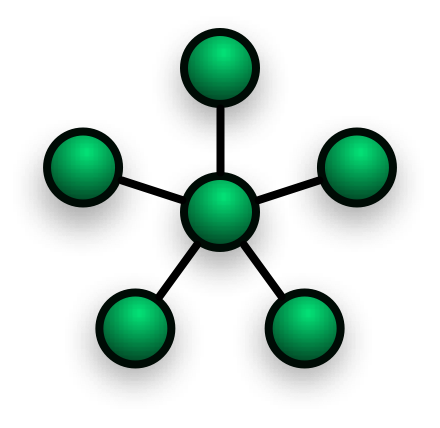
\includegraphics[width=\textwidth]{res/star.png}
      \caption{Star topology}
      \label{fig:star}
    \end{subfigure}
    ~
    \begin{subfigure}[b]{0.3\textwidth}
        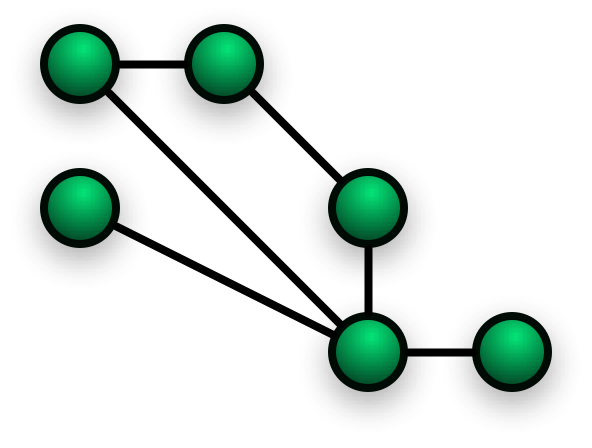
\includegraphics[width=\textwidth]{res/mesh.png}
        \caption{Mesh topology}
        \label{fig:mesh}
    \end{subfigure}
    \caption{Network topologies (Source: \href{en.wikipedia.org/wiki/Network_topology}{wikipedia.org})}
    \label{fig:topology}
\end{figure}

When designing our solution, the \textit{mesh network} was our main concern. The point-to-point and star topologies are quite easy to monitor as all traffic must pass through a known point. In the point-to-point, it would be on the two nodes that shares the connection, while in the star it would be the central hub. For the latter one, the star organization, we can consider the central hub to be a powerful device meaning it could be a netflow exporter if the need arises to analyze the network. But for the mesh topology, multiple distinct paths can exist for a node to reach another one. It is in need of an efficient solution. \\

After having discussed about the main topologies of IoT networks, we will now emphasize on what is called Wireless Sensor Networks, or WSN.


\subsection{Wireless Sensor Networks}

The main kind of IoT network we have focused on are Wireless Sensor Networks (WSN in shortened form). While our solution fits most types of IoT networks, we have decided to mainly focus on WSNs because they are the most constraining types.\\

As explained in \cite{vasseur2010interconnecting}, the idea behind \textit{Wireless Sensor Networks} is having small sensors collecting pertinent data from the physical world, communicating wirelessly to other sensors and in the end to a base station where all the data is collected and stored for further processing. Sensors not capable of directly transmitting information to the base station send their data to other sensors capable of relaying the information towards it, in a hop by hop fashion as illustrated in Fig.\ref{fig:wsn}. In that sense, WSNs present a mesh organization.\\

\begin{figure}
  \centering
  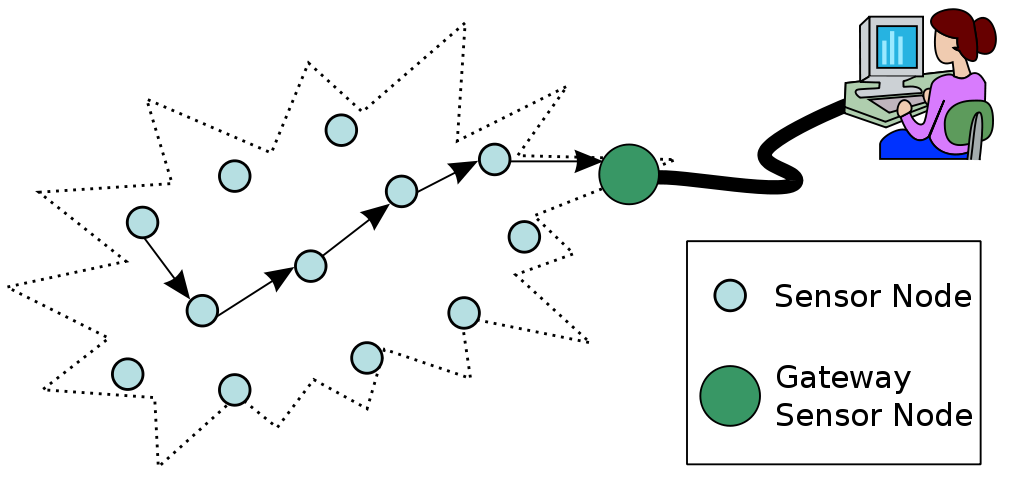
\includegraphics[width=\textwidth]{res/wsn.png}
  \caption{Wireless Sensor Networks (source: \href{commons.wikimedia.org/wiki/File:WSN.svg}{commons.wikimedia.org} )}
  \label{fig:wsn}
\end{figure}

Wireless Sensor Networks are regularly used for environmental conditions monitoring such as wild fire tracking, agriculture management, humidity and temperature monitoring in forests, effect of global warming on glacier structures, air pollution monitoring, and many more. They are also used in the industrial field such as in data centers, mainly to monitor the temperature of racks.  \\

The components of WSNs are "\textit{Wireless Nodes}" or "Motes" (see Fig.\ref{fig:xm1000}). WSNs may be composed of a few hundreds to thousands of nodes, each node being connected to one or several sensors. In addition to sensors, those nodes are also equipped with a microcontroller, a radio transceiver, memory, and a power source (eg. battery). The sensors are responsible for capturing data from the environment, especially when there is a change in an environmental condition such as temperature or humidity.  Sensors are usually very small and thus consume a very low amount of battery power. The \textit{microcontroller} is responsible for performing specific tasks and processing the data collected by the sensor, but also controlling other components of the node. The \textit{transceiver} is used for communication purposes, mainly sending and receiving data using specific. It is often of the form of a radio or infrared. Transceivers have the particularity of both being able to send and receive data. Finally, the \textit{power source} provides power supply instead of mains supply. The power source is thus in the form of a battery, it is consumed when the node is sending the environment, communicating with other sensor nodes, and doing some data processing. All of the components are designed to be as little power-consuming as possible. Having nodes not connected to mains power is an advantage thanks to not having to be plugged to a power supply (when the physical world makes it hard to have some, in moutains for example), but with such an advantage come resource constraints as we will explain later on.\\

\begin{figure}
  \centering
  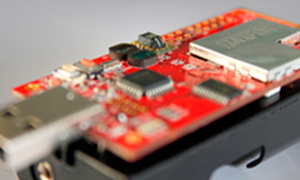
\includegraphics[width=0.5\textwidth]{res/xm1000.png}
  \caption{A AS-XM1000 sensor mote capable of sensing light, humidity and temperature (source: \url{www.advanticsys.com})}
  \label{fig:xm1000}
\end{figure}

The main challenges of WSNs are data transmission, resource constraint, and security. First, nodes must send their data to the server. As discussed earlier, each node may not have the server in their sending range because of a lack of power, thus they must send their data to an intermediate node relaying the information. Secondly, as stated before, the motes that composed a WSN present light components (weak CPU, small memory, etc). Moreover, because they are not plugged, they are quite limited in battery. Thus, they switch between \textit{idle} state and \textit{active} state, which also impacts data transmission as packets could be missed when sending on idle motes. Finally, the security issues are a consequences of the two first challenges. Because of the low characteristics of sensor nodes, it is difficult to implement security measures as sophisticated that on our laptops for example. This would drain the battery due to the added CPU usage. There would also be no sufficient memory to implement all those security measures.\\

\subsection{Radio Frequency IDentification - RFID}

Radio-frequency identification or RFID uses radio signals to record the presence of specific objects. Its purpose is the identification of a person or an item, using a system of tags. Tags are small transponders (combined radio receiver and transmitter). The transponders can transmit identity information when requested to. There also are tag readers to process the identification.\\

Tags are associated to products, animals, or people if their identification is needed for tracking for instance. The tracking is done using radio waves. There are two kinds of RFID tags, the active RFID tags that are battery-powered, and the passive RFID tags that have no batteries and work using signal power from other tags requesting information.\\

The RFID technology has a main advantage that is its limited cost and thus allow its deployment on a huge amount of devices.

\section{Challenges of The IoT}

IoT is still an emerging technology and need to resolve some challenges \cite{website:iot_challenge}. This section will be the occasion to discuss about such challenges that the IoT is confronted to.

\subsection{Lack of Standard Architecture}

The main challenges of the Internet of Things is to define a standard architecture \cite{abdmeziem2016architecting}. This is actually the main reason why it has not been fully deployed yet. Several characteristics are needed for the IoT to be deployed, and they should be included in the standard infrastructure. The characteristics needed are distributivity, interoperability (devices from different companies being able to communicate, with standardized protocols), scalability (huge amount of smart objects communicating), resources scarcity (power and consumption are limited on each device), and security.\\

Most existing applications using the Internet of Things have been developed privately. Companies, developers, researchers have developed some specific solutions using the Internet of Things. However, those solutions are more specific, and hence optimized, for one particular application.\\

\subsection{Three Aspects of The IoT Building Blocks}

As stated earlier, the introduction of the Internet of Things will mostly be an incremental integration to the current Internet. However, the \textit{IoT Building Blocks} is composed of three particular technologies that are crucial in the deployment of the IoT. First, there is the sensing technologies that are used to gather the interesting data. Then, there is what we call the middleware layer, that processes and manages the raw data gathered from the sensing technologies. Finally, there is the actuating technologies, corresponding to the physical extension of the IoT applications. We will take a look at the impact of these three notions on the future of the IoT.\\

The \textit{Sensing building block} plays an important role in data harvesting and communicating the data collected with sensors. Data is mostly transferred in a wireless fashion, in a Wireless Sensor Networks(WSN) organization or thanks to radio-frequency identification (RFID) because of their ability of sensing the environment. However, those organizations come with a few disadvantages such as security issues, reliability of wireless communication, and especially limited energy consumption that figures as a central obstacle to the deployment of WSNs and IoT networks. The limited availability of energy resources is an important matter to take care of. As a result, lightweight and energy-efficient routing protocols have been proposed but can only mitigate the energy limitation. \\

The \textit{Middleware building block} is a software interface that provides abstraction to hide heterogeneity of the technologies that are used in the Internet of Things and that may indeed differ from each other. Hence, the developers are exempted from having to know how the lower layer of the IoT works, and can primarly focus on the design of applications. \\

The middleware block could be taken care of by what we call \textit{Service-Oriented Computing} approches. A Service-Oriented architecture is a set of communicating services based on standardized interaction models. Associating Cloud Computing with a service-oriented architecture could actually provide an efficient middleware for the IoT. Sensor-clouds are of great help when it comes to handling huge loads of sensed data generated by sensing devices. Thus, approaches based on service lying on a cloud infrastrcuture introduces flexibility and adaptativity to middlewares for the IoT. The idea is to have the end users feel as if the physical sensors were virtually part of their physical resources (in their disk storage, or memory for example). In this case, the users do not need to know the location of the devices nor to know their location, and several end users from different companies developing different applications could exploit the sensors through the cloud. The cloud would thus provide sensor services to be exploited by different IoT applications. All these elements are key to developing IoT applications working on heterogeneous devices. \\

The \textit{actuating building block} finds its importance when it comes to making "dumb" objects "smart". Once the information is gathered from sensing in a specific situation, it is sent to the middleware infrastructure. After data processing from the middleware, a decision can be made through the actuator. In our e-health example discussed earlier where an ill person is equipped with an IoT node, in a hypoglycemia situation, the actuator could potentially save this person's life by automatically injecting sugar in the patient, the automation of the injection being faster than the wait needed for external intervention. \\

\subsection{Potential and Existing Architecture Design}

Though global architecture has yet to be decided in the Networking world, an architecture design has been proposed to be a base of the future global IoT architecture. \\

There is a three-layer architecture that is commonly accepted. It consists of the \textit{Perception Layer}, the \textit{Network Layer}, and the \textit{Application Layer}. \\

The \textit{Perception Layer} is used to sense the world via the sensors used in objects that are part of the IoT network. It uses technologies such as RFID and WSNs that we described earlier. This layer is also responsible for the conversion of the information into digital signals for transmission. The \textit{Network Layer} is where the processing of the data is done after collection through the Perception Layer, and it is responsible for the transmission of data to the application layer using network technologies such as WSN and LAN. In networks, the media for transmission may be 3G/4G, Wifi, or Bluetooth, to cite a few. The \textit{Application Layer} constitutes the front end of the IoT Architecture, it uses the processed data from the previous layers.\\

Even though no global standard infrastructure exists for the Internet of Things, some companies have nonetheless attempted to develop their own architecture, mainly for specific purposes answering to their local needs. There are usually two approaches for IoT Architectures, the first one is to use an existing architecture and adapt it to the IoT context, the second one is to create a new IoT architecture from scratch.\\

First, there is the \textbf{IETF protocol suite}. Considering the protocol stack of TCP/IP makes sense since it is widely deployed on the internet. However, applying it to the IoT context makes the deployment challenging because of resources scarcity of IoT devices, the instable wireless communication, and the heterogeneity of the traffic data and the devices. Knowing those difficulties, the IETF is trying to work with specific protocols of the IoT and standardizing them  for each layer of the stack. Namely, they use 802.15.4 \cite{molisch2004ieee} for the data link layer, 6LoWPAN \cite{montenegro2007transmission} (Low power Wireless Personal Area Networks) as the Network Layer for an addressing scheme, RPL \cite{winter2012rpl} (Routing Protocol for Low Power and Lossy Networks) as a routing protocol, and CoAP \cite{shelby2014constrained} (Constrained Application Protocol) as the application layer.\\

The \textbf{Server based approach}, called Server-Based Internet of Things Architecture. The idea behind this approach is to develop protocols and services based on a gateaway server such that the constrained devices in computation and communication capabilities are still part of the IoT in a secure and efficient way. For the \textit{physical and link layer}, each small device is connected to a single server, connecting the device and the internet and acting as a gateway. The \textit{Network Layer} is based on IPv6, by communicating with 6LoWPAN between the devices and the server. For the \textit{Transport Layer}, the server will comumunicate with the devices using UDP (UDP being lighter than TCP/IP) over 6LoWPAN. As for everything related to the application layer functions, the goal is to have each device offer a HTTP web-server interface for authorized users to use the functionalities of the said device. Those web-servers will be hosted on the gateway server.\\

As for creating a new IoT architecture from Scratch, a \textbf{Cloud Based approach} could be used. As we know, a considerable amount of data is generated from the devices. This data has to be stored and processed, as well as being retrieved in an efficient way. Cloud Computing aims at offering high reliability and scalability, along with providing data access for the IoT applications. A Cloud Computing platform for the IoT would thus receive the data collected from the sensors, analyze and intepret the data, as well as providing web visualizations. One advantage of the cloud is that it reduces the deploying costs for applications, but it is also scalable in essence. Indeed, sensing service providers can join the network and offer their data using a storage cloud, analytic tool developers can provide their software tools, artificial intelligence experts can provide their data mining and machine learning tools, and finally computer graphic designer can offer a variety of visualization tools.



%%%%%%%%%%%%%%%%%%%%%%%%%%%% IOT OS %%%%%%%%%%%%%%%%%%%%%%%%%%%%%%%%%%%%

\chapter{ContikiOS - Cooja}
\label{chap:contiki}

We will now discuss Operating Systems in the Internet of Things. As discussed earlier, objects in IoT Networks have limited capabilities, i.e. processing capacity and storage, and limited battery. It is thus preferred to have an operating system that is not demanding and as light as possible. \\

Though not ideal, a light version of Linux could be used. However, one requirement of working with smart objects is having the ability to react to \textit{Real-Time events}. In a situation where a smart sensor is used in a car to make its airbags open when a car crash occurs, the software in the said sensor must react to the crash almost instantly. In this case, we need a maximum time reaction to an event, otherwise the purpose of the object (and thus the airbag) is not met. A few operating systems have been developed to answer to the requirements of IoT objects \cite{website:iot_os}, they are light, have a minimal set of functionalities, plus they guarantee time-bounded reaction to events.\\

\section{The Contiki Operating System}

Among existing operating systems, we have chosen to use one that is called \textit{ContikiOS} \cite{website:contiki}. It is an open source operating system and it was developed in 2003. Contiki is quite light in terms of memory, processing speed, and communication bandwidth. Moreover, it is preemptive.\\

The reason we have chosen Contiki as OS for testing our idea is due to the simulation software, Cooja, which facilitates the debugging and the tests. Another reason, is that we are quite familiar with it having already programmed using Contiki. However, our solution should be easily ported to other OSs. The OS is just used to program the motes and as a proof of concept.\\

Contiki's main goal is to offer an OS for sensor nodes. Contiki applications are \textit{written in a subset of C} (example in Listing \ref{contiki_prog}) with a set of libraries written for Contiki purpose (memb for memory allocation for example). It is \textit{event-driven} as applications are mainly programmed by reacting to event. They use \textit{protothreads} which are "\textit{extremely lightweight, stackless threads that provides a blocking context on top of an event-driven system, without the overhead of per-thread stacks}" \cite{website:protothread}. Protothreads use the same stack, they only require two bytes of overhead by protothread and they cannot block when calling C functions. They offer advantages for embedded devices with small memory. \\

\begin{lstlisting}[language=C, frame=single, caption={Hello world program}, label=contiki_prog]
#include "contiki.h"
#include <stdio.h>
/*-----------------------------------------------------------*/
PROCESS(hello_world_process, "Hello world process");
AUTOSTART_PROCESSES(&hello_world_process);
/*-----------------------------------------------------------*/
PROCESS_THREAD(hello_world_process, ev, data)
{
  PROCESS_BEGIN();

  printf("Hello, world\n");

  PROCESS_END();
}
\end{lstlisting}

Contiki implements the recent IETF protocols for low-power IPv6 networking such as 6loWPAN and RPL. It provides three network mechanisms:
\begin{itemize}
\item uIP TCP/IP stack for IPv4 networking.
\item uIPv6 stack for IPv6 networking which is comprised of RPL and 6lowpan.
\item Rime stack which is an alternative to the two mentioned above.
\end{itemize}


\subsection*{Cooja Simulating Software}

\begin{figure}
  \centering
  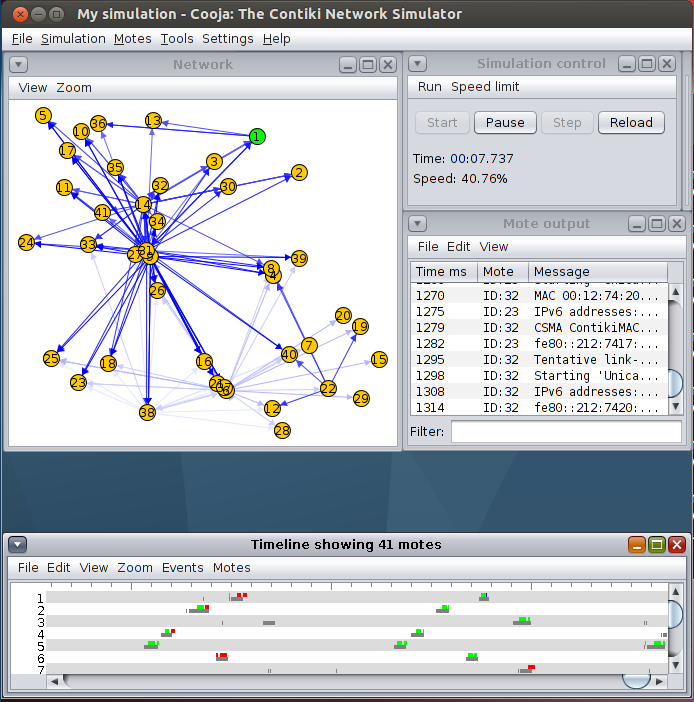
\includegraphics[width=0.5\textwidth]{res/cooja.png}
  \caption{Cooja a simulation software (Source: \href{commons.wikimedia.org/wiki/File:Contiki-ipv6-rpl-cooja-simulation.png}{commons.wikimedia.org})}
  \label{fig:cooja}
\end{figure}

An existing tool called \textit{Cooja} (see Fig.\ref{fig:cooja}) has been developed on Contiki. Cooja is a simulation software (partly an emulator too) for Internet of Things networks. It has many features, such as allowing to build networks with different types of components (Sky motes, Z1 motes). Those components are Contiki nodes, i.e. nodes working through ContikiOS. Cooja allows to upload code to virtual motes, the same way Contiki code may be uploaded on physical. Cooja can either emulate nodes (the hardware of each component is entirely emulated), or create "Cooja nodes" where Contiki code is uploaded on, compiled and then executed on a simulation host. Cooja allows to use non-Contiki nodes as well. Cooja presents itself as a very useful software for our thesis, as it allows us to simulate large networks, and is quite useful when it comes to testing, since the uploading and compilation time of Contiki codes on the nodes in the Network we are testing and analyzing is faster than on real hardware. It also avoids physical material restriction. One great aspect of Cooja is also that it offers to modify the environment to be, for example, more lossy, with higher transmission failure. It also disposes of useful plugins like a powertracker that keeps track of the amount of time a node send or receive messages.\\

With such a powerful simulation software, our decision to use the couple Contiki and Cooja was easy to take. Cooja was proven a useful tool to debug our code and analyze our solution.

\section{Others}

Contiki OS is not the sole Operating System for Internet of Things. There exist other ones with their advantages and disadvantages. Also, not all IoT OS have the same goal. Some focus on WSNs with low-power embedded devices while others have set their goals on more powerful devices. We will present some that retained our attention.

\begin{itemize}
\item \textbf{TinyOS}: Its first version was deployed in 2000. TinyOS \cite{website:tinyos} is an OS for low-power wireless embedded devices. It is event-driven like Contiki. It also presents a small memory footprint which is smaller than Contiki. It was written in NesC, a dialect of C.
\item \textbf{RIOT OS}: Developped in 2008, RIOT OS \cite{website:riot} \cite{baccelli2013riot} is an Operating System for Internet of Things. The goal of RIOT is to offer a platform to develop applications for the wide range of IoT devices. It presents a memory footprint of 1.5KB of RAM and 5KB of ROM. RIOT offers the possibility to write applications in C or C++. In contrary to Contiki which supports a subset of C, RIOT fully supports the C language with its standard libraries. It supports full multi-threading and real-time programming. Also in contrary to other IoT OSs, it offers hardware abstraction. Like Contiki, it supports the recent protocols of IETF like RPL, 6loWPAN and so on.
\item \textbf{Windows 10 IoT} \cite{website:win10} is the Operating System for IoT devices by Microsoft. It is an optimized version of Windows 10 for smaller devices like Raspberry Pi. However, it is not suited for WSN or small embedded devices as it needs a minimum of 256MB of RAM and 400MHZ processor to be effective.
\end{itemize}
%%%%%%%%%%%%%%%%%% MONITORING TOOLS %%%%%%%%%%%%%%%%%%%%%%%%%%%%%%%%%%%

\chapter{Monitoring tools}
\label{chap:monitoring_tools}

This chapter will be the occasion to present what has been done in the matter of monitoring tools for networks. The first section will be about the traditional networks and the second one will focus on the IoT networks.

\section{Traditional networks}

When speaking of monitoring for traditional networks, two techniques come to mind: \textit{Netflow} and \textit{sFlow}. The two approaches have the common goal to give network administrators informations about the traffic that passes through their networks. However, they differentiate in the way they do so. In our solution, we were mainly inspired by Netflow as it is lighter than sFlow in term of memory used.

\subsection{Netflow}

\textit{Netflow} is a feature that was created by Cisco Systems and introduced on Cisco Routers. Netflow allows the collection of the IP traffic in networks, and thus monitoring network traffic. Information such as Source and Destination addresses (defined as "Flows) and Traffic volume can be retrieved and further analyzed.\\

There are three components when having Netflow set up : the Flow Exporter, the Flow Collector(s), and the analysis application. The Flow Exporter collects packets and forms what we call flows (having various definitions according to the version of Netflow used). Flows represent a stream of packets sharing common attributes (such as source and destination addresses). The exporter records the flows into Netlow records and passes them onto the Flow Collector. After reception, the Flow Collector will store the flow records received from the Exporter. The data stored can then be analyzed by applications, hence having statistics of traffic exchanges in a particular network. This process is illustrated in Fig.\ref{fig:netflow}.\\

\begin{figure}
  \centering
  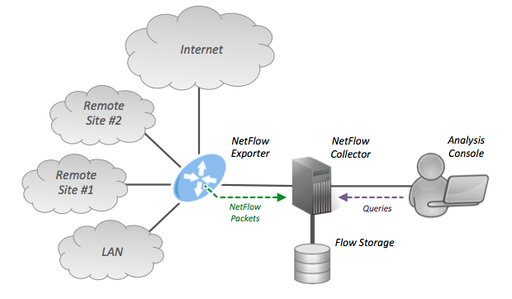
\includegraphics[width=\textwidth]{res/netflow.png}
  \caption{Netflow}
  \label{fig:netflow}
\end{figure}

The version of Netflow that we are quite interested in, is the Netflow version 10 or \textit{IPFIX} \cite{claise2013rfc}. This version is an IETF (Internet Engineering Task Force) protocol whereas the previous versions are proprietaty protocols of Cisco. IPFIX is template-based, meaning that contrary to previous versions of Netflow (excluded version 9 which is also template based), the netflow records can vary to suit the needs of the administrators or organizations. The template allows to define what we want to retrieve and by the same occasion define what we consider to be a flow. An organization could consider a flow to be 3-uple: source ipv6 address, destination ipv6 address, number of octets exchanged. While another one could consider a flow to be the 4-uple: source ipv6 address, destination ipv6 address, number of octets exchanged, number of packets exchanged. \\

The IANA (Internet Assigned Numbers Authority) has already defined some record fields like the Ipv6 source/destination address, the source transport port, and so on \cite{website:ipfix_entities}. However, the power of IPFIX lies in the possibility to define ourselves record fields (called entreprise fields). That is the main reason we were particularly interested in it. It is thus possible to for example define a record field for battery power remaining of the sender for. Furthermore, even if they suggest a size for record fields, they offer the possibility to redefine the size to a smaller one. The suggested field is only considered as an upper-bound, meaning we cannot propose a bigger size.\\

Having defined what Netflow is, the main goal here is to be able to use Netflow on an IoT device. In the Introduction section, we explained that our main goal was to analyze the traffic of an IoT Network and retrieve pertinent information such as the volume exchanged in the network, and its topology. Netflow is basically what we want to achieve in terms of data collecting. However, it has not been implemented by Cisco for IoT devices. Our task is to implement Netflow for an IoT device, using predefined data formats that will allow us to collect the information we are interested in (battery level, source and destination addresses, packet volume, etc.). In the Part \ref{part:solution}, we will describe in more details how we used Netflow in IoT networks as a solution to our monitoring task.

\subsection{sFlow}

\textit{sFlow} (for sampled flow) was initially proposed by the company HP. It is maintained by the sFlow.org consortium \cite{website:sflow}. The approach taken by SFlow is different than the one taken by Netflow. The two solutions share the notion of exporter, collector and analysis application. But the difference lies in the records that are sent by the exporter. \\

Whereas Netflow only sends information on the flows observed, sFlow sends original packets that pass through the network. sFlow is characterized by the \textit{polling interval} and the \textit{sampling rate}. The polling interval defines the periods at which the collector must report the number of occurences of packets that pass through. The sampling rate defines how much packets need to be sampled on a set number of packets. \\

The fact that exporters need to store packets makes this solution too heavy for majority of IoT devices. Another issue with sFlow is that we can miss peculiar packets by having a sampling rate different than 1:1 and thus lose important informations.

\section{IoT networks}

A plethora of tools exist to monitor Internet of Things networks. Yet, a preponderant part of those tools are data visualization centric. In this section, some tools will be presented. For a more exhaustive survey, see \cite{parbat2010data}.

\subsection{Octopus}

\textit{Octopus} \cite{jurdak2011octopus} is a software that allows to monitor and visualize WSN networks. It offers also the possibility to control those networks by giving command. The software was written in Java. \\

The GUI interface, Fig.\ref{fig:octopus_gui}, display a logical topology of the sensor nodes as well as charts reporting the retrieved values from the nodes. It also enables a user to modify the sampling rate at which nodes report the environmental values. \\

To effectively do so, Octopus needs the motes to send messages in a specific format so as to be able to parse them. The motes also need to be configured to be able to interpret messages coming from the software.\\

The architecture of Octopus, Fig.\ref{fig:octopus_archi}, is straightforward. The sensors nodes periodically send messages to a gateway which will be in charge of transmitting those messages to distant a Octopus client. The Scout can be seen as a collector that will listen for incoming messages. When it received a message, it will update the Mote DB who is in charge to maintain the status of the motes and also log the message. It will also trigger an update of the GUI interface, Panels. \\

\begin{figure}
    \centering
    \begin{subfigure}[b]{0.5\textwidth}
      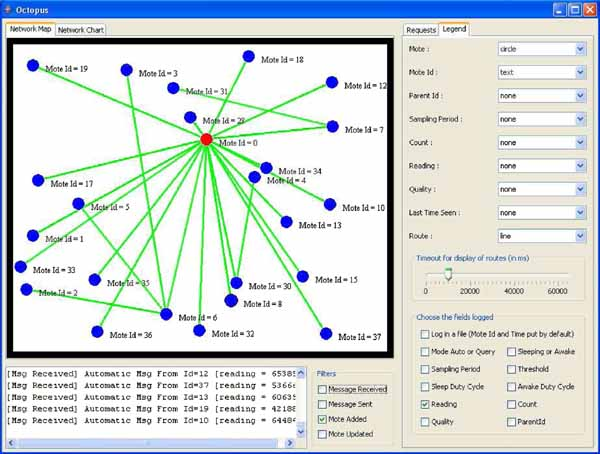
\includegraphics[width=\textwidth]{res/octopus.png}
      \caption{Octopus GUI}
      \label{fig:octopus_gui}
    \end{subfigure}
    ~
    \begin{subfigure}[b]{0.5\textwidth}
        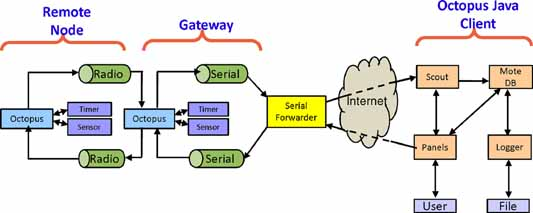
\includegraphics[width=\textwidth]{res/octopus_archi.png}
        \caption{Octopus architecture}
        \label{fig:octopus_archi}
    \end{subfigure}
    \caption{Octopus (Source: \href{www.researchgate.net/publication/220098661_Octopus_Monitoring_visualization_and_control_of_sensor_networks}{researchgate.net})}
    \label{fig:octopus}
\end{figure}

\subsection{Mote-View}

Mote-View \cite{turon2005mote} is a tool designed to simplify the administration of sensor networks (see Fig.\ref{fig:moteview}). They emphasize the visualization of data so as to be as user-friendly as possible. Mote-View is a client application. It offers the possibility to view the logical topology of nodes as well as their values. It provides  means to visualize the health of node which can be set based on different criteria such as the last time data was sent or the quality of link or congestion. An alert manager is made at the disposal of users to define their own alert conditions. Another feature is the conversion of different physical measurements units. \\

\begin{figure}
  \centering
  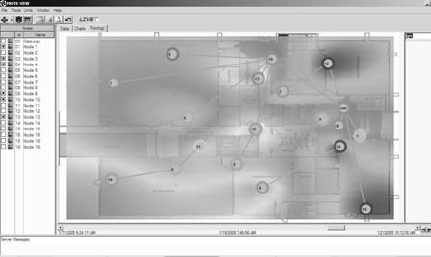
\includegraphics[width=0.6\textwidth]{res/moteview.png}
  \caption{Mote-View (Source: \href{www.researchgate.net/publication/4157258_MOTE-VIEW_A_sensor_network_monitoring_and_management_tool}{researchgate.net})}
  \label{fig:moteview}
\end{figure}

Mote-View is composed of four layers:
\begin{itemize}
  \item Data layer: mainly gives access to the database which store logs of the data sent by nodes.
  \item Node layer: stores the nodes status and also caches the results of queries done on the database.
  \item Conversion layer: applies the conversion of different units in the preferred choice of the user.
  \item Visualization layer: displays the data in form of graphs, topology, ...
\end{itemize}

Each layer offers abstraction and lets users make their own plug-ins to extend the functionalities of Mote-View. Mote-View can thus be viewed as a framework for monitoring tool for WSN.

\subsection{SensMap}

SensMap \cite{mraz2014visualization} is a web-based monitoring and visualization tool for sensor devices. It offers the possibility to display the nodes in three perspectives: Outdoor, Indoor and Topology. The Outdoor perspective display the locations of the nodes using Google maps. It leverages the possibility to display different nodes placed in different countries. The Indoor view shows the deployments of nodes inside a building (see Fig.\ref{fig:sensmap}). Finally, the Topology shows the logical topology of WSN.\\

Some features of SensMap are:

\begin{itemize}
  \item visualize the health of sensor devices;
  \item show the locations of nodes in three different perspectives as described before;
  \item display sensors data in real-time;
  \item show link quality between nodes;
  \item export data and much more.
\end{itemize}

The data that SensMap needs to be stored in the Xively public cloud \cite{website:xively}. This means that the sensor devices need to send their values to Xively. Then, SensMap will have access to them via the REST api offered by Xively.

\begin{figure}
  \centering
  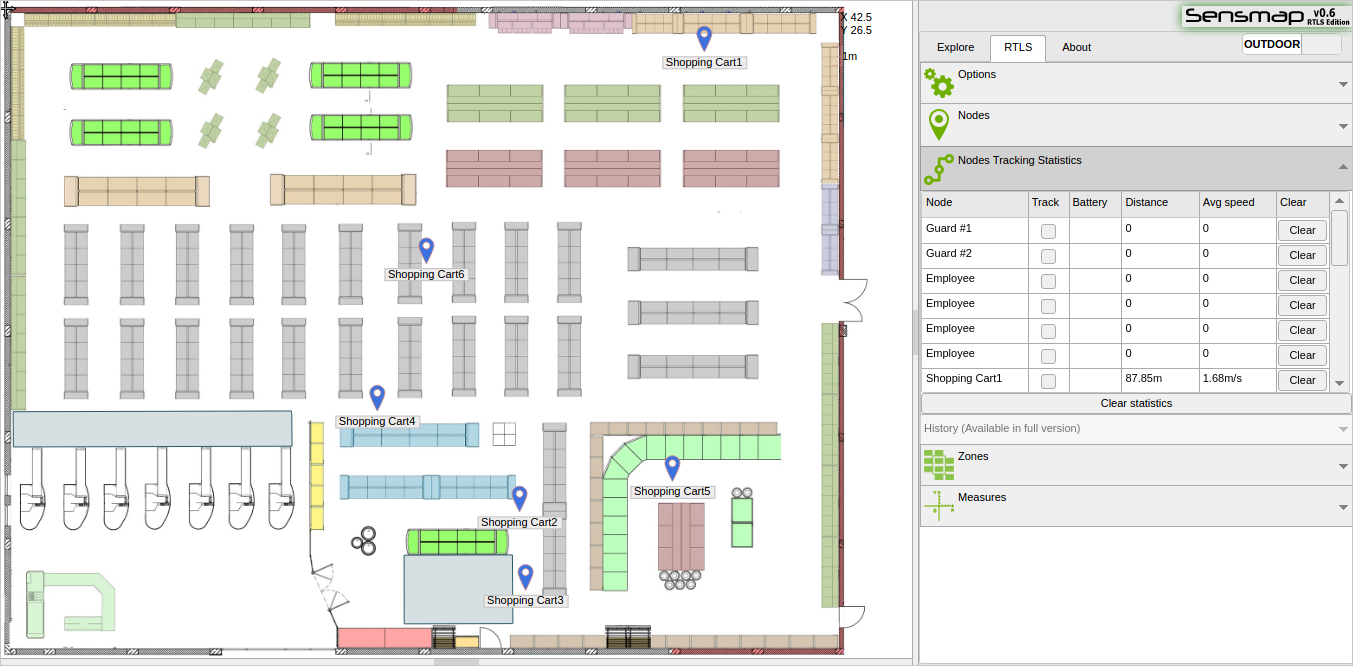
\includegraphics[width=\textwidth]{res/sensmap.jpg}
  \caption{Indoor perspective of SensMap}
  \label{fig:sensmap}
\end{figure}

\subsection{Foren6}

The approach taken by Cetic with their tool \textit{Foren6} \cite{website:foren6} is quite different than the other tools presented. Foren6 use sniffers to retrieve information of the network. Passive sniffers are scattered over the network and retransmit the traffic they observe. \\

The Fig.\ref{fig:foren6} shows the GUI interface of Foren6. Foren6 dispose of the following features:
\begin{itemize}
  \item Display logical topology of the motes.
  \item Analysis of previous records packet traces.
  \item Possibility to analyze simulated network like with Cooja.
  \item Exportation of data in pcap format. \\
\end{itemize}

\begin{figure}
  \centering
  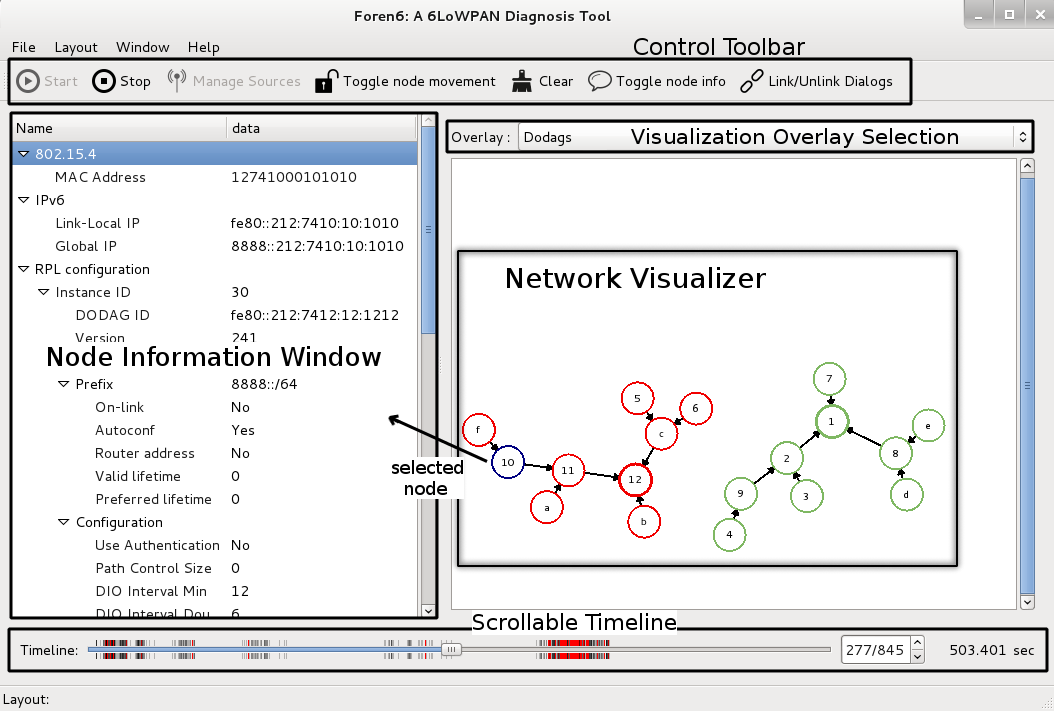
\includegraphics[width=\textwidth]{res/foren6.png}
  \caption{Foren6 GUI (source: \url{cetic.github.io/foren6/})}
  \label{fig:foren6}
\end{figure}

To be as efficient as possible, the solution offered by Cetic needs nodes to be solely focused on sniffing and also present enough processing power and battery to be able to sniff and transmit the packets captured. If the network is deployed on a large surface, there will be a need to have enough sniffers, well placed, so as to not miss traffic. Also should those motes, sniffers send the packets captured using the other IoT nodes, it would increase the burden on the network. \\

\subsection{Tiny IPFIX}

TinyIPFIX \cite{schmitt2016tinyipfix} is not a monitoring tool but a technique. It was designed as to retrieve the sensors values as main goal. TinyIPFIX is a light version of the IPFIX protocol which was discussed before.\\

TinyIPFIX works by having the sensors nodes play the role of exporters. They export their values in the TinyIPFIX format which will be translated into IPFIX format by the gateway. The TinyIPFIX format is essentially the same as the original IPFIX format only that a compression of the message header is done. By means of this, the original header size of 20 bytes can be reduced to 3 bytes, saving 17 bytes.\\

One big advantage of TinyIPFIX is that by using templates like IPFIX, users can define their own templates depending on the values they want to retrieved. Another asset is that messages that go out of the IoT network are in IPFIX format. Organizations using already IPFIX to monitor their network do not need to modify their infrastructure.

\subsection{Discussion}

Most of the monitoring solutions for Internet of Things networks are essentially client applications. All of them focus on Wireless Sensors Networks and essentially visualization of the readings of the sensors networks. However, apart from the Foren6 solution that exports the data from nodes in pcap format, the others impose their own specific format of data or simply do not state the format they intend to receive. But our guess is that they also require their own format of message so as to be able to understand the data received. This means that users or organizations disposing of administration infrastructures need to severely update them to make use of those tools. \\

The drawbacks of having such disparity of format for data are that users cannot switch freely between those tools, nor they have the convenience to use multiple tools at the same time. The motes would need to be reprogrammed to deliver new data format. Plus, it would impose too much charge on them if they had to send their values in multiple format. One solution would be to have a service that reformat data in the desired format but it would not resolve the problem. There is a need for a protocol that would suit the need of all organizations in the values that they would like to retrieve. This is why our attention was focused on \textit{TinyIPFIX}, as we consider it to be the solution to this particular issue. \\

As stated before, majority of the tools focused on showing the readings of the sensors. In that sense, they do not give information about how traffic is generated by the network. We cannot detect abnormal behaviors such as nodes contacting a surprising number of other nodes. We also lack statistics to improve our network. For instance, by knowing that a certain node is highly solicited we can replace it by a more powerful device. Organizations, if not already, will be in need of powerful tools to diagnose their networks in order to correct issues more rapidly or improve the efficiency of their networks. Our monitoring tool has as a goal to solve this issue and provide meaningful insights about IoT networks. \\

However, all those tools share some common functionalities which must be considered as a basis when developing new such softwares. One important functionality is the display of logical topology of the motes showing the links formed between the motes. Another feature is the storing of the data for later analyzing. One other common requirement is the modularity of those tools and the ease to produce plug-ins. Those basic functionalities should be included when designing such softwares.
